\documentclass[article]{jss}
\usepackage{amsfonts,thumbpdf}

\newtheorem{lemma}{Lemma}
\newtheorem{theorem}{Theorem}
\newtheorem{corollary}{Corollary}
\newtheorem{example}{Example}
\newtheorem{proposition}{Proposition}
\newtheorem{definition}{Definition}
\newtheorem{conjecture}{Conjecture}
\newtheorem{assumption}{Assumption}
\def\logit{\mathop{\rm logit\,}\nolimits}
\def\midd{\mathop{\,|\,}\nolimits}
\def\defn{{\stackrel{\rm def}{=}}}
\def\eqdistn{{\stackrel{\cal D}{=}}}
\newcommand{\bea}{\begin{eqnarray}}
\newcommand{\eea}{\end{eqnarray}}
\newcommand{\beaa}{\begin{eqnarray*}}
\newcommand{\eeaa}{\end{eqnarray*}}
\newcommand{\qed}{{\rule{2mm}{2mm}}}
\newcommand{\en}{{\rule{.75em}{0cm}}}
\newcommand{\svskip}{\vspace{.125in}}
\newcommand{\mvskip}{\vspace{.25in}}
\newcommand{\lvskip}{\vspace{.5in}}
\newcommand{\R}{\mathbb{R}}

\def\vec#1{\mathchoice{\mbox{\boldmath$\displaystyle\bf#1$}}
{\mbox{\boldmath$\textstyle\bf#1$}}
{\mbox{\boldmath$\scriptstyle\bf#1$}}
{\mbox{\boldmath$\scriptscriptstyle\bf#1$}}}

\title{\pkg{ergmuserterms}: A Template Package}
\Plaintitle{ergmuserterms: A Template Package}
\Shorttitle{\pkg{ergmuserterms}: A Template Package}

\author{
  David R.\ Hunter \\ Penn State University \And
  Steven M.\ Goodreau \\ University of Washington \And
  Mark S.\ Handcock \\ University of California, Los Angeles
}
\Plainauthor{David R. Hunter, Steven M. Goodreau, Mark S. Handcock}

\Abstract {
Abstract here
}
\Keywords{
exponential-family random graph model, Markov chain Monte Carlo, maximum likelihood estimation, p-star model}

%\Volume{}
%\Issue{}
%\Month{}
%\Year{}
%\Submitdate{}
%\Acceptdate{}

\Address{
David R.\ Hunter \\
Department of Statistics \\
Pennsylvania State University \\
University Park, PA 16802, United States of America\\
E-mail: \email{dhunter@stat.psu.edu} \\
URL: \url{http://www.stat.psu.edu/~dhunter/}
}

\begin{document}

\section{Introduction}
\label{introduction}

At the core of the \pkg{ergm} package \citep{ergm}
for \proglang{R} \citep{r2010}
is a sophisticated
Markov chain Monte Carlo engine for simulating random networks.
As explained by \citet{ergmjss}, simulating a Markov chain on a
set of networks
whose stationary distribution is given
by the exponential-family random graph model
\bea\label{ergm}
P_{\vec\theta_0} (\vec Y = \vec y) =
\frac{ \exp\{ \vec \theta_0^\top  \vec g(\vec y) \} }
{ \kappa(\vec\theta)}
\eea
is vitally important not only for simulation but also for estimation.
In equation (\ref{ergm}), $\vec\theta_0\in \R^p$ is a fixed parameter vector,
$\vec g(\vec y)$ is a user-defined $p$-vector of statistics on the
network $\vec y$ assumed to come from some set ${\cal Y}$ of networks, and
\bea\label{kappa}
\kappa(\vec\theta) = \sum_{\vec z \in {\cal Y}} \exp\{ \vec \theta_0^\top  \vec g(\vec z) \}
\eea
is the normalizing constant.

The MCMC scheme implemented in \pkg{ergm} is called a Metropolis-Hastings
algorithm.  In general terms, such an algorithm proceeds from step $t$ to step $t+1$,
from one network $\vec y^k$ to the next, by (a) selecting a candidate
for the next network $\vec y^{k+1}$, (b) computing a {\em Hastings ratio} based on
$\vec y^k$ and the candidate network, and (c) deciding whether $\vec y^{k+1}$
should be set to the candidate network or, alternatively, whether to stay put
for another iteration and set $\vec y^{k+1}=\vec y^k$.
The selection (a) is done so that any possible network, say $\vec z$, has probability
$q(\vec z, \vec y^k)$ of being selected, where $q$ is some probability function known
to the user.  (The $q$ function can and, in general, does place probability zero on
some values of $\vec z$, depending on the value of $\vec y^k$.)
The Hastings ratio (b) is equal to
\begin{equation}\label{hastings}
\frac{P_{\vec\theta_0} (\vec Y=\vec y^k)}{P_{\vec\theta_0} (\vec Y=\vec z)}
\frac{q (\vec y^k, \vec z)}{q (\vec z, \vec y^k)},
\end{equation}
where $\vec z$ is the candidate network selected in (a).  Finally, (c) is done by selecting
a real number, say $u$, uniformly from the unit interval (0,1) and comparing $u$ with
the Hastings ratio.  Then
\[
\vec y^{k+1} = \cases{\vec z & if $u \le \mbox{Hastings ratio}$; \cr
\vec y^k & if $u>\mbox {Hastings ratio}$.}
\]
In particular, note that if the Hastings ratio is greater than one, the candidate $\vec z$ is
always accepted as the value for $\vec y^{k+1}$.

In \pkg{ergm}, there are different possible choices of the probability distribution $q(\vec z, \vec y_{t})$
used to select $\vec z$, but for the most part they all limit the possible choices of $\vec z$
to those that differ from $\vec y^k$ by exactly one edge indicator;  in other words, $\vec z$
involves a single edge toggle of $\vec y^k$.  Suppose that $\vec z$ is identical to $\vec y^k$
in all except the $(i,j)$ entry.  Notationally, we would write $x_{ij}=1-y_{ij}^k$ but
$\vec z_{ij}^c=\vec (y^k_{ij})^c$, where $\vec z_{ij}^c$ denotes the entire network $\vec z$
{\em except for} the $(i,j)$ entry.  In this case, by substituting Equation~(\ref{ergm}) into
Expression~(\ref{hastings}), we see that the Hastings ratio may be simplified to
\begin{equation}\label{hastings2}
\frac{q (\vec y^k, \vec z)}{q (\vec z, \vec y^k)} \exp\{\pm \vec\theta_0^\top \delta (\vec y^k)_{ij} \},
\end{equation}
where
\begin{equation}\label{changestats}
\delta (\vec y)_{ij} \stackrel{\rm def}{=} \vec g(\vec y_{ij}^+) - \vec g(\vec y_{ij}^-)
\end{equation}
denotes the {\em vector of change statistics}, found by subtracting the two vectors of
$\vec g$-statistics evaluated at the networks formed by leaving all of $\vec y$ unchanged
except for the $(i,j)$ entry, which is set to 1 in $\vec y_{ij}^+$ and 0 in $\vec y_{ij}^0$.
The sign of the $\vec\theta_0^\top \delta (\vec y^k)_{ij}$ term
in~(\ref{hastings2}) depends on the value
of $y_{ij}^k$:  If $y_{ij}^k=1$, then the term gets a plus sign; otherwise it gets a minus.

The key conclusion of all of the above development is that the calculation of
change statistic vectors is of vital importance to the running of both the simulation and
the estimation routines in the \pkg{ergm}.   While the \pkg{ergm} package itself provides
a large library of possible change-statistic calculation routines \citep{ergmtermsjss},
individual users sometimes wish to estimate or simulate from a model that
includes specialized statistics not among those already coded in the \pkg{ergm}
package; to do so, it is necessary for them to write code to calculate the
associated change statistics for the Metropolis-Hastings algorithm.
This article describes an \proglang{R} package called
\pkg{ergmuserterms} that is designed to make this process as straightforward as possible.
It also explains some of the internal workings of the \pkg{ergm} package that will
help users develop their own network change statistic code.

In Section~\ref{syntax}, we discuss the unique syntax implemented in the \pkg{ergm}
package and explain why it was necessary to extend the existing formula-based
syntax (as used, say, by the \code{lm} and \code{glm} functions in \proglang{R})
to handle models of the form found in Equation~(\ref{ergm}).

\section[Syntax for a call to the ergm function]{Syntax for a call to the \code{ergm} function}
\label{syntax}

A traditional generalized linear model, as explained in the classic book by
\citet{mccullaghnelder1989}, consists of a specification of the probabilistic dependence
of some {\em response} variable, usually denoted $Y$, on some
function of a linear combination of some other {\em predictor} variables,
usually denoted $X$.  The distribution of $Y$ is generally a member of some
known exponential family;
In its simplest form (ignoring any dispersion parameters), we may write the
density or mass function of $Y$, which depends on some
parameter vector $\vec\phi$, as
\[
f_Y(y) = \exp\{ \vec a(y)^\top \vec b(\vec\phi) - c(\vec\phi) \}.
\]
Standard exponential family theory \citep[e.g.,][]{brown1986fse}
reveals that $E(Y) = (\partial / \partial\vec\phi) c(\vec\phi)$.
In a generalized linear model, we presume that
\[
E(Y) = \mbox{link}(\vec X^\top \vec\beta)
\]
for some ``link'' function.  Implicit in this formulation is the
fact that $\vec X$ in considered a fixed quantity, independent of $Y$;
indeed, $\vec X$ is often termed the {\em independent} variable.
(Even when $\vec X$ is random, one typically specifies a generalized
linear model for the conditional distribution of $Y$ given $\vec X$, so
that $\vec X$ may be considered constant in this context.)

In contrast, model~(\ref{ergm}) does not in general conform to the above
specifications of a generalized linear model.  While it is true that the distribution of
the network $\vec Y$---the ``response''---is expressed in exponential family
form, there is no way to specify some fixed $\vec X$ and some link function so that
$E(\vec Y)= \mbox{link}(\vec X^\top \vec\beta)$.  Essentially, this is because
an ERGM involves an inherent auto-dependence between the ``response'' and
any traditional notion of the ``predictors''.

In addition, there is
no closed-form expression for the likelihood function in an ERGM that
can be easily evaluated.  Equation~(\ref{ergm}) is generally impossible
to use for the purposes of calculation due to the fact that
the $\kappa$ function of Equation~(\ref{kappa}) involves an enormous number
of summands for even simple networks.  Thus, even the estimation methods
necessitated by maximum likelihood estimation for an ERGM differ from those
used by a generalized linear model.  In the former case, we rely on MCMC
sampling to generate an approximation to the likelihood, whereas in the
latter the likelihood may be evaluated, and thus maximized, directly.

%Because an ERGM is not a generalized linear model,
%it is not possible to use exactly the same \proglang{R} syntax used for
%\code{glm} calls  in order to specify a call to \code{ergm}.
Let us consider a typical call to the \code{glm} function in \proglang{R}:
\begin{CodeChunk}
\begin{CodeInput}
R> glm ( response ~ predictor1 + predictor2 + predictor3, link = binomial)
\end{CodeInput}
\end{CodeChunk}
In a general ERGM, there
is no way to define \code{predictorX},
nor is there a closed-form way to relate the expected value of the random
network to the linear combination of the network statistics.  Thus, there is
no way to specify a link function and the standard \proglang{R} formula
(that is, \code{response ~ predictors}) does not apply.  Nonetheless, there
are still analogies to standard regression models, so the
\code{ergm} function was designed to employ a modified version of the
standard \proglang{R} formula:
\begin{CodeChunk}
\begin{CodeInput}
R> ergm ( network ~ netstat1 + netstat2 + netstat3)
\end{CodeInput}
\end{CodeChunk}
Numerous examples of calls to the \code{ergm} function may be found in
\citet{ergmjss} and \citet{statnettutorialjss}, and a list of numerous possibilities
for \code{netstatX} is given in \citet{ergmtermsjss}.

{\bf Remark:\ }
For certain choices of the vector $\vec g(\vec y)$ of graph statistics, the resulting
model~(\ref{ergm}) actually implies that all of the individual $y_{ij}$ edge indicators
are jointly independent.  In these cases, model~(\ref{ergm}) is actually equivalent
to a logistic regression model, which {\em is} a generalized linear model.
See Section~3 of \citet{HunGoodHan08} for more details on these so-called
independence models.
{\em Is there a better reference than this?  Maybe it would be better to expand a bit and
describe how ergm actually finds the MPLE for a typical ergm call.}


\section[Network storage in ergm]{Network storage in \pkg{ergm}}
\label{networkstorage}

Because an understanding of the internal storage of a network in the
\pkg{ergm} package will aid the writing of code for a change
statistic, we describe this storage in some detail here.
A network with $n$ nodes is
internally represented in \pkg{ergm} as a set of $2n$ edgelists,
$n$ for ``in-edges'' and $n$ for ``out-edges''.  If the directed edge $(3,5)$ exists in the network,
then we call 3 the ``head'' node and 5 the ``tail'' node of this edge.  We would say that node 5 is
on an out-edge from node 3 and that node 3 is on an in-edge to node 5.  Thus, the 3rd out-edge list
should contain 5 and the 5th in-edge list should contain 3.  Naturally, this scheme results in
redundancy, and maintaining these two sets of edgelists entails both a storage and a performance
cost.  However, in situations where an algorithm must be able to look up both all in-edges and all
out-edges of a node, this scheme is very efficient.
In the case of an undirected network, the designations of ``head'' and ``tail'' are arbitrary, and we
define the smaller-numbered node as the head and the larger-numbered
node as the tail.

Storage of each node's in-edge list and out-edge list is implemented using a standard
binary tree structure
as in \cite[Chapter 13]{algorithms}.  This structure allows for efficient lookup, insertion, and deletion
operations that typically take $O(\log d)$ time, where $d$ is the degree, or number of neighbors, a
particular node has.  In a binary tree such as those shown in Figure \ref{outedgefig},
each parent node has two potential children, with the left child's value always less than the
parent's and the right child's value always greater.  To avoid the worst-case performance
that can result from a list of values being passed in strictly increasing or decreasing order,
each node's edgelist is randomly permuted before it is stored as a tree.

\begin{figure}[htb]
\vspace{3ex}
$\displaystyle{\pmatrix{
 0 & 0 & 1 & 0 & 0 & 1 & 0 & 1 \cr
 0 & 0 & 0 & 0 & 1 & 0 & 0 & 0 \cr
 0 & 0 & 0 & 0 & 0 & 1 & 1 & 1 \cr
 0 & 1 & 0 & 0 & 1 & 0 & 1 & 0 \cr
 1 & 1 & 1 & 1 & 0 & 0 & 0 & 0 \cr
 1 & 1 & 0 & 0 & 0 & 0 & 0 & 1 \cr
 0 & 0 & 0 & 0 & 0 & 0 & 0 & 0 \cr
 1 & 0 & 1 & 0 & 1 & 0 & 0 & 0 }
 }\qquad\qquad\vtop{\vskip-15ex \hbox{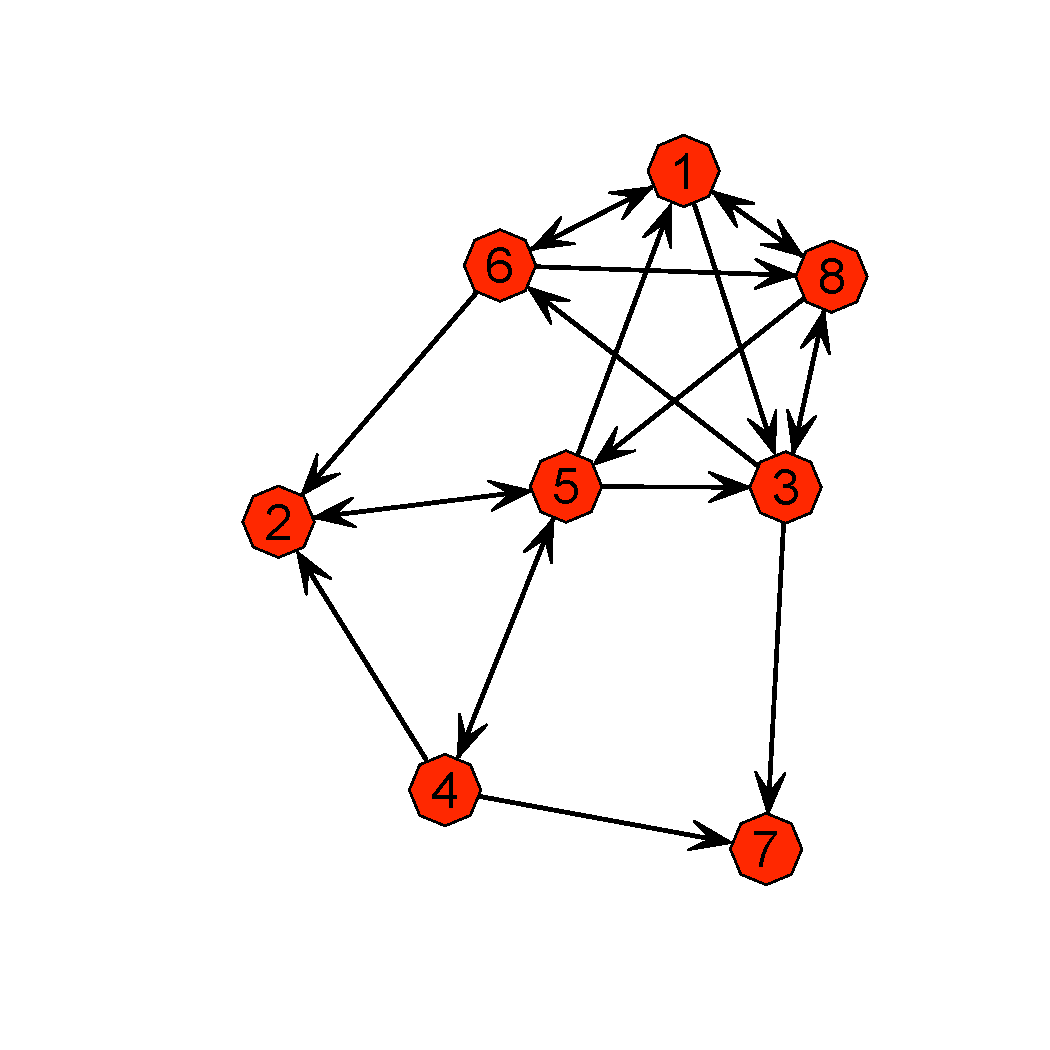
\includegraphics[height=2in, width=2in]{net8nodes.pdf}}}
$
\caption{The adjacency matrix (on left) and a corresponding graphical representation
of a directed 8-node network.  The rows of the adjacency matrix define
the out-edge lists of Figure \ref{outedgefig}.}\label{8nodeexample}
\end{figure}

\begin{figure}[htb]
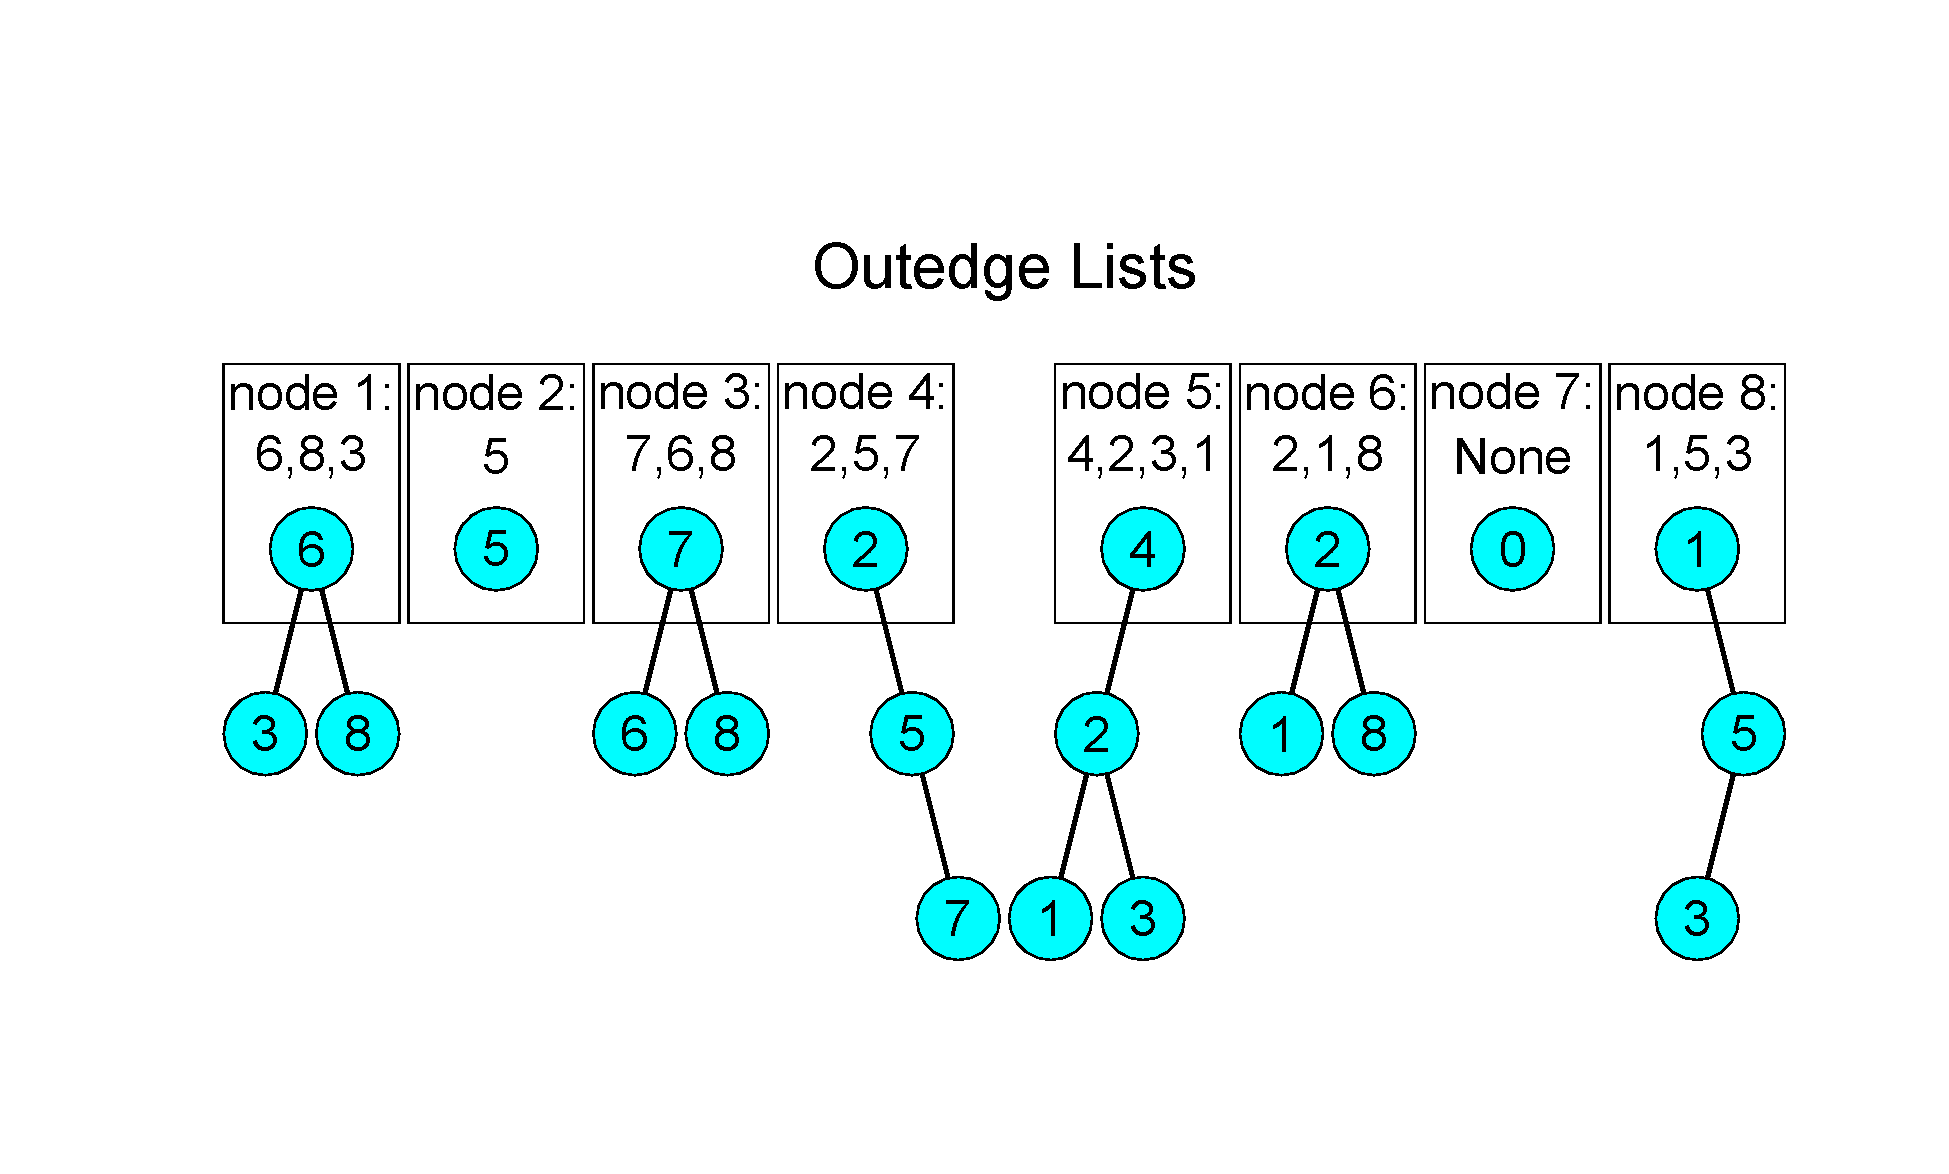
\includegraphics[height=2in, width=4in]{outedgelists.pdf}
\caption{This is the resulting internal representation of the out-edges for the network of
Figure \ref{8nodeexample}.  Each node's out-neighbors are permuted randomly
before the binary trees are built.}\label{outedgefig}
\end{figure}

The binary tree routines, all written in the C language, are contained in the
\code{src/edgetree.c} file in the \pkg{ergmterms} package (the \pkg{ergm} package
includes the same code).  These routines may be used to initialize or destroy
a network object, to manipulate that object by adding or deleting edges, and to
query that object to ascertain the presence of an edge.
The \code{NetworkInitialize} and \code{NetworkDestroy} functions
are used internally by the \pkg{ergm} package to create a network object
and destroy it when it is no longer needed by the C code.  These two functions
are not generally called by the user, though interested users may find it interesting
to look at them.  Also, the definition of the \code{Network} type, in the
\code{src/edgetree.h} file, reveals that a network keeps updated lists of every node's
in- and out-degree in addition to the actual edges.  A user may exploit these statistics
when writing code for various change statistics as described in Section \ref{Cside}.

\section{Acquiring and setting up the necessary tools}
\label{Tools}

Coding new change statistics for \pkg{ergm} requires two steps that users might not have previously encountered: building an \proglang{R} package from source, and writing and compiling \proglang{C} code. These steps requires additional tools beyond those needed by most \proglang{R} end users; in this section we walk through the process of acquiring and setting up such tools. Those users who are already familiar with this task may wish to skip ahead to Section~\ref{Rside}.

\subsection{Acquiring tools for Windows}
\label{ToolsWindows}

Windows users will need three tools: Perl, CLT and MinGW.\footnote{This list of necessary tools is current as of this writing. The authoritative and up-to-date source for the set of tools necessary is Appendix D (``The Windows Toolset'') of the \proglang{R} Installation and Administration manual (\url{http://cran.r-project.org/doc/manuals/R-admin.html\#The-Windows-toolset})} The easiest way to acquire all three is through the website Building \proglang{R} for Windows (currently at \url{http://www.murdoch-sutherland.com/Rtools}), which also provides an excellent overview of the process described in this section.  Simply download the latest version of \code{RtoolsXX.exe} from this website, and install.  While doing so, be sure to check ``Edit the system PATH''; allow it to edit your path so that \code{c:\textbackslash Program Files\textbackslash Rtools\textbackslash bin}, \code{c:\textbackslash Program Files\textbackslash Rtools\textbackslash perl\textbackslash bin}, and \code{c:\textbackslash Program Files\textbackslash Rtools\textbackslash MinGW\textbackslash bin} are up front. After these three entries, insert an additional entry containing the bin directory of your current \proglang{R} installation.  This is typically \code{C:\textbackslash Program Files\textbackslash R\textbackslash R-X\textbackslash bin}, where \code{X} is your \proglang{R} version number.


\subsection{Acquiring tools for MacOS}
\label{ToolsMac}

?

\subsection{Acquiring tools for Unix}
\label{ToolsUnix}

?

\subsection[Obtaining source code for the ergmuserterms package]{Obtaining source code for the \pkg{ergmuserterms} package}
\label{Source}

When one is planning only to use an \proglang{R} contributed package as-is and not edit the source code, one need only install and load it using the \code{install.package} and \code{library} commands, respectively.  When wishes to edit the content, one must download the source code, and then build from there. For all operating systems, one should:

\begin{enumerate}
\item Go to the contributed packages page on CRAN. Dave: this will be on CRAN before we release the paper, right?
\item Select \pkg{ergmuserterms}.
\item Select the source code file (with extension \code{tar.gz}) next to ``Package Source''.
\item Save this file in \code{R-working-directory\textbackslash src\textbackslash library}.  Be very careful not to place it in \code{R-working-directory\textbackslash library}. In fact, you can technically place the file anywhere on your machine, as long as it is not in \code{R-working-directory\textbackslash library}.  In Windows, your \proglang{R} working directory will typically be \code{C:\textbackslash Program Files\textbackslash R\textbackslash R-X}, where \code{X} is your \proglang{R} version number). (MacOS? Unix?)
\item Untar the file.  For Windows you can do this by opening a DOS window (\code{Start>Run} and type \code{cmd}), navigating to the folder where you just saved the source code file, and typing \code{tar xfz name.of.sourcecode.file} (MacOS? Unix?) A directory named \code{ergmuserterms} will be extracted in your current directory.
\end{enumerate}

\subsection[Building ergmuserterms]{Building \pkg{ergmuserterms}}
\label{BuildEUT}

Windows users: In a DOS window, go to the same directory where you saved the \pkg{ergmuserterms} source file in the previous step, and type:

\code{RCMD INSTALL ergmuserterms}

(MacOS? Unix?)

You can now load the basic \pkg{ergmuserterms} package into \proglang{R} with the \code{library(ergmuserterms)} command.

In Sections~\ref{Rside} and~\ref{Cside} we will describe the process of editing the R and C code to make new statistics.  Any time you have made changes that you want to see incorporated into the version of \pkg{ergmuserterms} that you are using in \proglang{R}, simply repeat the instructions in this section.

\section[Writing change statistics using ergmuserterms:  The R side]%
{Writing change statistics using \pkg{ergmuserterms}:  The R side}
\label{Rside}

A typical call to the \code{ergm} function might look like this:
\begin{CodeChunk}
\begin{CodeInput}
R> ergm ( network ~ edges + degree(1:3) + absdiff("age"))
\end{CodeInput}
\end{CodeChunk}
We refer to \code{edges}, \code{degree}, and \code{absdiff} as {\em terms}.
In the \pkg{ergm} package, there are roughly 70 terms (as of this writing) available.
Documentation for these terms is
 in \citet{ergmtermsjss} and is also available by typing \code{help(ergm-terms)}.
 Terms may take arguments, such as the vector \code{1:3} or the nodal covariate
 name \code{"age"} above.  Implementing a new term that can be used by
 the \code{ergm} function involves adding two functions:  One written in \proglang{R}
 and one written in \proglang{C}.  This section describes the former, while Section \ref{Cside}
 describes the latter.
 
The \proglang{R} function, whose purpose is to initialize the internal representation
of the model term  just after a call to the  \code{ergm} function,
must be called \code{InitErgmTerm.termname}.  It should have a specified format and should
perform certain tasks.  We will examine these by considering the
\code{absdiff} term:
\begin{CodeChunk}
\begin{CodeInput}
 InitErgmTerm.absdiff <- function(nw, arglist, ...) {
  ### Check the network and arguments to make sure they are appropriate.
  a <- check.ErgmTerm(nw, arglist, directed=NULL, bipartite=NULL,
                      varnames = c("attrname","pow"),
                      vartypes = c("character","numeric"),
                      defaultvalues = list(NULL,1),
                      required = c(TRUE,FALSE))
  ### Process the arguments
  nodecov <- get.node.attr(nw, a$attrname)
  ### Construct the list to return
  list(name="absdiff",
       coef.names = paste(paste("absdiff", if(a$pow != 1) a$pow else "",
       pkgname = "ergmuserterms",
       sep = ""), a$attrname, sep = "."), 
       inputs = c(a$pow, nodecov),
       dependence = FALSE )
}
\end{CodeInput}
\end{CodeChunk}
The \code{absdiff} term has one required argument, called \code{attrname}, and
one optional argument, called \code{pow}.  This term will add to the
model a network statistic equal to 
\[
\sum_{i,j} y_{ij} |X_i-X_j|^p,
\]
where $X_i$ and $X_j$ are the values of the nodal covariate named \code{attrname}
(and assumed already to be part of the network object specified in the
\code{ergm} function call) and $p$ is the value of \code{pow}.  By default, \code{pow}
is one.  

We now examine the \code{InitErgmTerm.absdiff} function line by line:
\begin{itemize}
\item[Line 1:]
Any \code{InitErgmTerm} function must take three arguments: 
\code{nw}, \code{arglist}, and \code{...}.  The first of these will be the network object, from
which any necessary information may be extracted.  The second, \code{arglist},
will be the list of arguments passed by the user of the term, if any.  Finally, \code{...}
is necessary primarily for backward compatibility, as some existing InitErgmTerm arguments may
be passed additional arguments, and without the \code{...} this could generate an error message.
\item[Line 3:] 
The call to the \code{check.ErgmTerm} function should be performed by every 
\code{InitErgmTerm} function, and its result is typically given the name \code{a}.  
The first two arguments to \code{check.ErgmTerm} are the network and argument list; these
should not be modified.  However, the \code{directed} and \code{bipartite} arguments may
be set to \code{TRUE} or \code{FALSE} if the term should only be applicable to the specified 
types of networks.  (An error results if a term is not appropriate, for example, if a directed network
is used in a call with a term for which \code{directed=FALSE}.)  Leaving \code{directed=NULL}
and \code{bipartite=NULL} indicates that the term may be used on either directed or 
undirected, either bipartite or unipartite networks.
\item[Line 4:]  Each argument to a term has a name, and these names are
specified by \code{varnames}.  The \code{check.ErgmTerm}
function will return a list in which each item is named corresponding to the its varname.
In the example, the list will have items named \code{attrname} and \code{pow}.
In the case of a term with no arguments (such as \code{edges}), use 
\code{varnames=NULL}.
\item[Line 5:] In this example, the argument \code{attrname} is of type
\code{character} and the argument \code{pow} is of type \code{numeric}.
\item[Lines 6 and 7:] The \code{attrname} argument is required; i.e., an error results
if the user does not specify this argument.  Therefore, the default \code{NULL} is
irrelevant.  However, since \code{pow} is not required, its value will be set to the 
default of 1 whenever the user does not supply it.
\item[Line 9:] This line extracts a vector of nodal covariate 
values from the network object.  The name of this covariate was passed in by the
user and is the character string called \code{attrname} in the list returned by the
\code{check.ErgmTerm} function.
\item[Line 11:]  Each \code{InitErgmTerm} function should return, upon exit,
a list whose items are all named.  Some names are required, and some
are optional.  A full list of these is given in the header of the \code{InitErgmTerm.users.R}
file in the \code{R} subdirectory of the \pkg{ergmuserterms} package.  
The first named item shown here, \code{name}, is required.  It gives the name 
of the C function (when ``\code{d_}'' is prepended) that will calculate the
change statistic(s) for this term; see Section \ref{Cside} for details.  In this case,
we know that the function \code{d_absdiff} will be responsible for this calculation.
\item [Lines 12 and 13:]  The \code{coef.names} is another required element in the output
list (the only one other than \code{name}).  It should give a vector of names
for the statistic(s) that are to be added to the model by this term.  The present
example adds only a single statistic whose name contains 
both \code{absdiff} and the name of the nodal attribute, along with the exponent
\code{pow} if it is not one.  The length of the vector of statistic names determines how
many statistics \pkg{ergm} will expect the term to add to the model.
\item [Line 14:]
The \code{pkgname} is the name of the \proglang{R} package in which the 
\proglang{C} function that calculates change statistics can be found.  By default,
this is \pkg{ergm}, but for new terms defined in the \pkg{ergmuserterms} package
the default must be overridden.
\item [Line 15:]
Because \code{absdiff} relies on the values of a nodal covariate, these values must be available to 
the C function that calculates the change statistic.  In addition, the value of the
\code{pow} exponent must be available to the change statistic function.  All these values
are concatenated into a single numeric vector and given the name \code{inputs} in the
list.
\item[Line 16:]  The \code{dependence=FALSE} means that this term does not, by itself, 
result in an ERGM in which the dyads are dependent.   If all terms in a model 
have \code{dependence=FALSE} set, then the entire model is a dyadic independence
model.  By default, if \code{dependence} is omitted then it is assumed \code{TRUE}.
\end{itemize}
One additional item that can go
in the output list is \code{emptynwstats}, which is a vector of the
same length as the number of statistics generated by the term being added.  This vector 
gives the value of the network statistic measured on a network with no edges.  The reason for
this is that the empty network gives a point of reference for calculating global values of the statistics using \proglang{C} code that only calculates change statistics.  
By default, \code{emptynwstats} is a vector of zeros, so it is only necessary to include this
item for cases where the empty network does not have the value zero for some of the statistics.
For instance, the \code{isolates} term counts the number of zero-degree nodes in the network,
and this statistic equals $n$ when the network is empty; thus, the \code{InitErgmTerm.isolates}
function ends with the following lines:
\begin{CodeChunk}
\begin{CodeInput}
  list(name="isolates",
       coef.names = "isolates",
       emptynwstats = network.size(nw) )
\end{CodeInput}
\end{CodeChunk}

Other items that can go into the 
output list are described in the comments at the top of the
\code{InitErgmTerm.users.R} file in the \code{R} subdirectory of the \pkg{ergmuserterms}
package.  Those not described above deal with curved exponential family models,
which we do not discuss here; nonetheless, the reader is encouraged to read the 
comments at the top of the \code{InitErgmTerm.users.R} file.

Any \code{InitErgmTerm} function will be automatically included in the \pkg{ergmuserterms}
package if it is saved in a file ending with the extension \code{.R} in the \code{R} subdirectory.
For instance, a user may simply use a text editor to add new \code{InitErgmTerm}
functions to the existing \code{InitErgmTerm.users.R} file, then these
functions will automatically be incorporated into the \pkg{ergmuserterms}
package.

\section[Writing change statistics using ergmuserterms:  The C side]%
{Writing change statistics using \pkg{ergmuserterms}:  The C side}
\label{Cside}

{\it Note to Steve (and myself):  The examples that are currently part of the R/InitErgmTerm.R and
src/changestats.c files are not necessarily the best ones, and they are not the same
as the absdiff example I wrote about in this article.  Probably we should change 
these examples.}


As explained at the beginning of Section \ref{Rside}, adding a term to be
used with the \pkg{ergm} package requires two different functions:  An 
\code{InitErgmTerm} function written in \proglang{R} and a
change statistic function written in \proglang{C}.  This section discusses the
second of these, which should be placed in a file with the extension \code{.c} 
in the \code{src} directory, just as the examples in the 
\pkg{ergmuserterms} package are found in the \code{changestats.c}
file.
Any \code{.c} file placed in the \code{src} subdirectory in the 
\pkg{ergmuserterms} package will
automatically be compiled when the package is installed from source.

Readers familiar with writing \proglang{C} code may at first not recognize 
the example \code{d_absdiff} function shown below.  This is because it
uses numerous macros, named using all capitals
in the \code{changestats.h} file in the
\code{src} directory, that are designed to make writing change statistic
functions easier.
For instance, an author of the \code{absdiff} term need not worry about 
the arguments that will be required of the \code{d_absdiff} function; these
are automatically included by typing 
\code{D_CHANGESTAT_FN(d_absdiff)}.  Here, \code{D_CHANGESTAT_FN} is a macro
defined to create a new function whose name is supplied by the user and 
whose arguments agree exactly with the arguments that will automatically be passed to 
it by the \pkg{ergm} package.

Here, then, is the code for the \code{d_absdiff} statistic:
\begin{CodeChunk}
\begin{CodeInput}
D_CHANGESTAT_FN(d_absdiff) { 
  double change, p; Vertex h, t; int i;
  ZERO_ALL_CHANGESTATS(i);
  FOR_EACH_TOGGLE(i) {
    h = heads[i]; t = tails[i]; 
    p = INPUT_ATTRIB[0];
    if(p==1.0){
      change = fabs(INPUT_ATTRIB[h] - INPUT_ATTRIB[t]);
    }else{
      change = pow(fabs(INPUT_ATTRIB[h] - INPUT_ATTRIB[t]), p);
    }
    CHANGE_STAT[0] += IS_OUTEDGE(h,t) ? -change : change;
    TOGGLE_IF_MORE_TO_COME(i); /* Needed in case of multiple toggles */
  }
  UNDO_PREVIOUS_TOGGLES(i); /* Needed on exit in case of multiple toggles */
}
\end{CodeInput}
\end{CodeChunk}
Following the first line, various variables are declared.  The \code{Vertex} type 
is a safe way to declare any integer variables that may be as large as the total number of
vertices in the network; there is also a similar \code{Edge} type.
After the variable declarations, essentially every change statistic function has the following
form:
\begin{CodeChunk}
\begin{CodeInput}
  ZERO_ALL_CHANGESTATS(i);
  FOR_EACH_TOGGLE(i) {
    /* body of function */
    TOGGLE_IF_MORE_TO_COME(i); /* Needed in case of multiple toggles */
  }
  UNDO_PREVIOUS_TOGGLES(i); /* Needed on exit in case of multiple toggles */
\end{CodeInput}
\end{CodeChunk}
The \code{body} of the change statistic function has the goal of
updating the \code{CHANGE_STAT} vector, which has entries
\code{CHANGE_STAT[0]}, \ldots, 
\code{CHANGE_STAT[N_CHANGE_STATS-1]},
as appropriate for the $i$th toggle specified by 
\code{heads[i]}, \code{tails[i]}.  The logic is that the proposal could possibly involve
multiple edge toggles, and the job of the change statistic function is to update the
change statistics as appropriate for the entire set of toggles.
Since some of the macros, such as \code{ZERO_ALL_CHANGESTATS} and 
\code{FOR_EACH_TOGGLE}, 
 require the use of a variable (such as \code{i} in the code above), it is important
 that this variable be declared as type \code{int} prior to its first use.
 
Inside the \code{FOR_EACH_TOGGLE(i)} loop, the value of \code{i} 
counts from 0 to \code{ntoggles-1}, where \code{ntoggles} is the total number of
toggles being considered.  In each case, the proposed toggle is to the
directed edge (\code{heads[i], tails[i]}).  Even when the network is considered undirected,
every edge is stored as a directed edge from the ``head'' node to the ``tail'' node.  
After initially zeroing all of the change statistics using the
\code{ZERO_ALL_CHANGESTATS} macro, the function should, for each edge 
toggle propsed, calculate how the toggle would change the network statistics of the
network.  This is a subtle difference here as compared to  the $\delta(y)_{ht}$ function of 
Equation~(\ref{changestats}), where the change is always calculated as the edge $(h,t)$ 
changes from 0 to 1.  In a change statistic function in \pkg{ergm}, however, the sign of the
change will depend on whether the proposed toggle is to an existing edge or not.

We may see how this is done by examining the body of the \code{d_absdiff} function below.
Remember that \code{h} and \code{t} are variables of type \code{Vertex} (which is essentially
the same as type \code{int}), whereas \code{p} and \code{change} are of type
\code{double}:
\begin{CodeChunk}
\begin{CodeInput}
    h = heads[i]; t = tails[i]; 
    p = INPUT_ATTRIB[0];
    if(p==1.0){
      change = fabs(INPUT_ATTRIB[h] - INPUT_ATTRIB[t]);
    }else{
      change = pow(fabs(INPUT_ATTRIB[h] - INPUT_ATTRIB[t]), p);
    }
    CHANGE_STAT[0] += IS_OUTEDGE(h,t) ? -change : change;
\end{CodeInput}
\end{CodeChunk}
When the \code{inputs} item was added to the output list of the
\code{InitErgmTerm.absdiff} function, it consisted of a single
real number, the exponent, followed by a value of some nodal attribute
for each of the $n$ nodes.  These inputs may be accessed now as the
\code{INPUT_PARAMS} vector, which has entries
\code{INPUT_PARAMS[0]} through \code{INPUT_PARAMS[N_INPUT_PARAMS-1]}.
Thus, the first step in the body of our change statistic function is to read the value of
the exponent (\code{INPUT_PARAM[0]}), then calculate the absolute value of the
difference of the nodal attributes for the nodes numbered \code{h} and \code{t},
for these are the nodes involved in the proposed toggle.  If necessary (i.e., 
if \code{p} is not one),
the absolute difference is raised to the appropriate power.  
The change statistic---there is only one change statistic, 
\code{CHANGE_STAT[0]}, in this case---will then be equal to plus or minus
the exponentiated absolute difference, depending on the value
returned by the \code{IS_OUTEDGE} macro.  In Section \ref{networkstorage},
we explained that each node's full list of in-edges and out-edges is constantly
updated.  Therefore, each edge is listed in two places, so that if the
edge \code{(h,t)} is currently in the network, both 
\code{IS_OUTEDGE(h,t)} and \code{IS_INEDGE(t,h)} would return one
rather than zero.  In this case, it suffices to check whether \code{(h,t)} is
an outedge:  If it is, then the toggle would remove the edge and so 
we should add \code{-change} to \code{CHANGE_STAT[0]}; otherwise,
we should add \code{change}.

In some change statistic functions, it is necessary to look at all of the current
neighbors of a particular node.  The macros
\code{STEP_THROUGH_OUTEDGES} and \code{STEP_THROUGH_INEDGES}
can help with this.  Each of these macros takes three arguments; suppose
we call them $(a, e, v)$.  The first argument (which should be declared to of type \code{Vertex}) is the node whose in- or out-edges
we wish to examine.  The second argument (of type \code{Edge}) is the looping
variable that steps through each of the neighbors of \code{a} in turn.  Finally,
the third variable (of type \code{Vertex}) is set by the macro to equal the number of
the node corresponding to the edge.  It is important to remember that for undirected
networks, each edge is only stored as $(h,t)$, where $h<t$.  Therefore, to step
through all of the edges of node \code{h} in an undirected network, it is necessary
to step through all of its in- and out-edges by using
\code{STEP_THROUGH_OUTEDGES(h, e, v)}
followed by 
\code{STEP_THROUGH_INEDGES(h, e, v)}.  It is possible to observe
examples of these macros in the \code{changestats.c} file in the
\pkg{ergm} package.

Other macros are described briefly in the file \code{changestats.h} in the \code{src}
directory.  Again, many examples of the use of these macros are available in the
\code{changestats.c} file.


\section{Examples}
\label{Examples}

{\em Steve: Write this!}

\section*{Acknowledgments}

{\em Billy.}

\bibliography{v24}

\newpage

\begin{appendix}


\section[appendix]{Appendix}
\label{appendix}

\end{appendix}

\end{document}
